\documentclass[../TG_magistrsko_delo_sections.tex]{subfiles}
\graphicspath{{\subfix{../images/}}}

\begin{document}
V prejšnjem poglavju smo obravnavali periode zveznih preslikav definiranih na dveh disjunktnih intervalih in na krožnici. Ko smo obravnavali periode poljubne funkcije $f$ definirane na prostoru $X = I_1 \cup I_2$, smo prišli do relacije $\triangleright_X$, ki določa prisotnost period za preslikavo $f : X \to X$. Natančneje, če je $m$ perioda za zvezno preslikavo $f:X \to X$, potem je vsako naravno število $l$, za katero je $l \triangleleft_X m$, tudi perioda za preslikavo $f$. V tem poglavju bomo obravnali prostore, pri katerih je relacija, ki določa prisotnost period preslikave enaka relaciji Šarkovskega, ki smo jo spoznali v definiciji~\ref{def:ureditev-sark}. Če je relacija $\triangleright_X$ enaka relaciji Šarkovskaga, pravimo, da je prostor $X$ \emph{prostor Šarkovskega}. V tem poglavju, bomo spoznali nekaj prostorov Šarkovskega in tudi nekaj prostorov, ki to niso. S primeri in protiprimeri bomo poskušali ugotoviti katere topološke lastnosti imajo prostori Šarkovskega.
Preden začnemo s preučevanjem različnih prostorov Šarkovskega se prepričajmo, da je lastnost biti prostor Šarkovskega topološka lastnost. 
\begin{trditev}
Lastnost biti prostor Šarkovskega je topološka lastnost. To pomeni, če je $X$ prostor Šarkovskega in je prostor $Y$ homeomorfen prostoru $X$, potem je tudi $Y$ prostor Šarkovskega.
\end{trditev}
\begin{proof}
Naj bo prostor $X$ prostor Šarkovskega in naj bo prostor $Y$ homeomorfen prostoru $X$. Naj bo $h : X \to Y$ homeomorfizem med prostoroma $X$ in $Y$. Preslikavi $f : Y \to Y$ in $g = h^{-1} \circ f \circ h : X \to X$ imata enake periode, zato je $Y$ tudi prostor Šarkovskega.
\end{proof}

%Nove prostore, ki so prostori Šarkovskega, lahko poiščemo tudi s pomočjo nekaterih zveznih preslikav. Definirajmo tako preslikavo, ki nam pomaga konstruirati nove prostore Šarkovskega.

%\begin{definicija}
%Naj bo $X$ topološki prostor in $A \subseteq X$ njegov podprostor. Zvezni preslikavi $r : X \to A$ pravimo \emph{retrakcija}, če je preslikava $r|_A = id_A$. Podprostor $A \subseteq X$ je \emph{retrakt} prostora $X$, če obstaja retrakcija $r: X \to A$.
%\end{definicija}

%S pomočjo retrakcije lahko pridemo do novih prostorov Šarkovskega.

%\begin{trditev}
%Retrakt prostora Šarkovskega je prostor Šarkovskega.
%\end{trditev}
%\begin{proof}
%Denimo, da je prostor $X$ prostor Šarkovskega in prostor $A \subseteq X$ retrakt prostora $X$. Naj bo $r : X \to A$ retrakcija $i : X \to A$ inkluzija. Če je funkcija $f : A \to A$ zvezna, ima funkcija $g = i \circ f \circ r : X \to X$ enake periodične točke, kot funkcija $f$. Zato je tudi prostor $A$ prostor Šarkovskega.
%\end{proof}

Iz prejšnjih poglavji je razvidno, da so tipični predstavniki prostorov Šarkovskega množica realnih števil in intervali v realnih številih. V poglavju~\ref{sec:circ} smo spoznali dva prostora, ki nista prostora Šarkovskega. Največ časa smo namenili krožnici, ki ni prostor Šarkovskega, saj imajo na primer pri rotaciji za $120^\circ$ vse točke periodo $3$, drugih period pa ta rotacija nima.
S podobnim sklepanjem lahko za nekatere prostore hitro preverimo, da niso prostori Šarkovskega. To naredimo tako, da poiščemo kakšno os $n$-kratne rotacijske simetrije, kjer je $n$ naravno število večje od $2$. Pri takih primerih lahko hitro ugotovimo, da ima rotacija za kot $\varphi = \frac{360^\circ}{n}$, za $n>2$, točke periode $n$ in morda tudi točke periode $1$, nima pa točk periode $2$. Zaradi tega taki prostori ne morejo biti prostori Šarkovskega. Primeri takih prostorov so npr. sfera, krogla, torus \dots 


Na začetku poglavja~\ref{sec:circ} smo enostavno pokazali, da disjunktna unija dveh intervalov ni prostor Šarkovskega. Z zelo podobno idejo lahko pokažemo, da je vsak prostor Šarkovskega povezan.

%\begin{definicija}
%Topološki prostor $X$ je \emph{nepovezan}, če obstajata neprazni odprti podmnožici $U, V \subset X$, ki zadoščata spodnjima pogojema:
%\begin{enumerate}
%\item $U \cup V = X$ in 
%\item $U \cap V \neq \emptyset$.
%\end{enumerate}
%Prostor, ki ni nepovezan je \emph{povezan}.
%\end{definicija}

\begin{trditev}
Prostor Šarkovskega je povezan.
\end{trditev}
\begin{proof}
Naj bo prostor $X$ disjunktna unija nepraznih prostorov $A$ in $B$ in naj bosta $a \in A$ in $b \in B$ poljubni točki tega prostora. Definiramo preslikavo $f:X \to X$ s predpisom:
\[ f(x) = \begin{cases}
  a, & \mbox{ če $x \in B $}\\
  b ,& \mbox{ če $x \in A$.}
  \end{cases}
  \]
Preslikava $f$ ima samo dve periodični točki. To sta točki $a$ in $b$. Obe pa imata periodo 2. Ker nobena točka prostora $X$ ni fiksna točka za preslikavo $f$, prostor $X$ ni prostor Šarkovskega.
\end{proof}

Pokazali smo, da je vsak prostor Šarkovskega povezan prostor. V nadaljevanju bomo ponovili kakšni prostori so s potmi povezani, lokalno povezani in lokalno s potmi povezani. S primeri se bomo prepričali, da obstajajo prostori Šarkovskega, ki imajo te lastnosti, in tudi prostori Šarkovskega, ki teh lastnosti nimajo.

%Najbolj tipični primeri prostorov Šarkovskega so intervali v realnih številih. Ti so povezani s potmi, lokalno povezani in lokalno povezani s potmi. Poglejmo si primer prostora Šarkovskega, ki ni 

\begin{definicija}
Topološki prostor $X$ je \emph{s potmi povezan}, če za poljubni točki $a, b \in X$ obstaja zvezna preslikava $\gamma:[0, 1] \to X$, za katero je $\gamma(0) = a$ in $\gamma(1) = b$. Preslikavi $\gamma$ rečemo tudi pot med točkama $a$ in $b$.
\end{definicija}

Primeri s potmi povezanih prostorov so intervali v realnih številih, krožnica, disk v $\R^2$\dots
\begin{trditev}
Lastnost biti s potmi povezan je strožji pogoj, kot biti povezan. To pomeni, da je vsak s potmi povezan prostor tudi povezan.
\end{trditev}

\begin{dokaz}
Naj bo $X$ s potmi povezan prostor. Dokazovali bomo s protislovjem. Denimo, da prostor $X$ ni povezan. Potem obstajata neprazni odprti množici $U, V \subseteq X$, za kateri veljata naslednji lastnosti:
\begin{enumerate}
\item $U \cup V = X$ in 
\item $U \cap V = \emptyset$.
\end{enumerate}
Množici $U$ in $V$ sta neprazni, zato si lahko izberemo točki $a\in U$ in $b\in V$. Prostor $X$ je s potmi povezan, kar pomeni, da obstaja pot $\gamma : [0, 1] \to X$, za katero je $\gamma(0) =a$ in $\gamma(1)=b$. Sedaj bomo obravnavali množici $\gamma^{-1}(U)$ in $\gamma^{-1}(V)$. Množici sta disjunktni podmnožici intervala $[0, 1]$, njuna unija pa je enaka interevalu $[0, 1]$. Obe množici sta odprti v $[0, 1]$, saj je pot $\gamma$ zvezna preslikava. Ker je $0$ element množice  $\gamma^{-1}(U)$ in $1$ element množice $\gamma^{-1}(V)$, tvorita ti dve množici separacijo povezane množice $[0, 1]$, kar je protislovje. Torej je prostor $X$ povezan.
\end{dokaz}

Implikacija v drugo smer ne drži. Torej, če je nek topološki prostor $X$ povezan, ne moremo sklepati, da je tudi s potmi povezan. Poglejmo si primer povezanega prostora, ki pa ni s potmi povezan.

\begin{definicija}
Naj bo $C$ grapf funkcije $\sin\left(\frac{\pi}{x}\right)$ na intervalu $x \in (0 , 1]$ in naj bo $A$ daljica $\{ 0 \} \times [-1 , 1]$. \emph{Varšavski lok} je prostor homeomorfen prostoru $X = C \cup A$.
\end{definicija}

\begin{figure}[h]
  \centering
  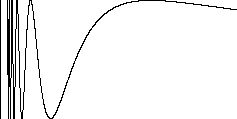
\includegraphics{varsavskilok.pdf}
% \caption[caption za v kazalo]{Dolg caption pod sliko}
  \caption[Primer vektorske slike.]{Varšavski lok.}
  \label{fig:varsavski_lok}
\end{figure}


Komponenta $A$ je homeomorfna zaprtemu intervalu $[-1, 1]$, komponenta $C$ pa je homeomorfna polodprtemu intervalu $(0, 1]$. Denimo, da lahko množico $X$ zapišemo kot unijo dveh nepraznih disjunktnih odprtih množic $U$ in $V$. Ker je množica $C$ povezana, celotna leži v eni množici, denimo, da leži v množici $V$. Pokažimo, da v vsaki okolici točke $x = (0, 0) \in  A$ ležijo tudi točke iz množice $C$ in zato tudi iz množice $V$. Naj bo $\delta$ poljubno majhno pozitivno število in množica $D = B(x, \delta) \cap X$ delta okolica točke $x$ v prostoru $X$. Za naravno število $k > \frac{1}{\delta}$ točka $\left(\frac{1}{k}, 0\right)$ leži v množici $C$ in v množici $D$, kar pomeni, da točka $(0, 0)$ leži v množici $V$. Ker je množica $A$ povezana množica, cela leži v množici $V$. Ugotovili smo, da celoten prostor $X$ leži v množici $V$, zato je povezan prostor.

Pokažimo, da varšavski lok ni s potmi povezan. Predpostavimo, da obstaja pot $p$ med točkama $(0, 0) \in A$ in $(1, 0) \in C$, za katero velja $p(0) = (0, 0)$ in $p(1) = (1, 0)$. Naj bo $x: \R^2 \to \R$ projekcija na os $x$. Funkcija $x$ je zvezna. Pot med točkama $(0, 0)$ in $(1, 0)$ se začne na množici $A$ in mora v neki točki ,,skočiti'' na množico $C$, ki je del varšavskega loka s pozitivno koordinato $x$.   
Definiramo natančen čas, ko se to zgodi kot število $t_0$:
$$t_0 := \inf\{t \in [0, 1]: x(p(t)) > 0 \}.$$
Za vsako število $t < t_0$ je $x(p(t)) = 0$. Zaradi zveznosti funkcije $x \circ p$ v točki $t_0$ velja enakost $x(p(t_0)) = \lim\limits_{t \uparrow t_0} x(p(t)) = 0$. Zaradi zveznosti preslikave $p$ lahko izberemo tako pozitivno realno število $\delta$, za katerega velja:
$$t_0 \leq t < t_0 + \delta \Rightarrow ||p(t) - p(t_0)|| < \frac{1}{2}.$$
Obstaja točka $t_1 \in (t_0, t_0 + \delta)$, za katero je $a := x(p(t_1)) >0$. Ker je množica $[t_0, t_1]$ povezana, je tudi njena slika $x(p([t_0, t_1]))$ z zvezno funkcijo $x \circ p$ povezana in vsebuje $0 = x(p(t_0))$ in $a = x(p(t_1))$. Vsaka povezana podmnožica množice realnih števil $\R$ je interval, zato velja:
$$[0, a] \subseteq x(p([t_0, t_1])).$$

\begin{figure}[h]
  \centering
  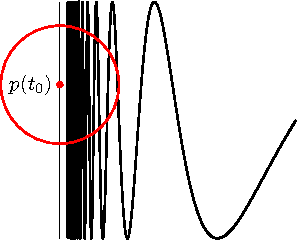
\includegraphics{varsavski_lok_s_potmi_nepovezan.pdf}
% \caption[caption za v kazalo]{Dolg caption pod sliko}
  \caption[Primer vektorske slike.]{Skica dokaza, da varšavski lok ni s potmi povezan prostor.}
  \label{fig:varsavski_lok}
\end{figure}

S slike lahko razberemo, da je to v protislovju z zveznostjo funkcije $x \circ p$, saj graf funkcije $\sin\left(\frac{\pi}{x}\right)$ sega izven rdečega kroga s središčem v $p(t_0)$. Zato $x$-vrednosti točk na množici $X$, ki ležijo znotraj kroga, ne vsebujejo vseh vrednosti iz intervala $[0, a]$. Pretvorimo vizualno razlago v matematični dokaz.

Za $k > \frac{2+a}{4a}$ ležita števili $\frac{2}{4k+1}$ in $\frac{2}{4k-1}$ v intervalu $[0, a]$. Ti dve števili predstavljata $x$-koordinati točk $p(t')$ in $p(t'')$ za neki števili $t', t'' \in [t_0, t_0 + \delta)$. Velja $p(t') = (\frac{2}{4k+1}, 1)$ in $p(t'') = (\frac{2}{4k-1}, -1)$. Zaradi izbire števil $t'$ in $t''$ iz intervala $[t_0, t_0 + \delta)$ in zaradi zveznosti preslikave $p$, velja $||p(t') - p(t_0)||< \frac{1}{2}$ in $||p(t'') - p(t_0)||< \frac{1}{2}$ iz česar sledi, da je $||p(t') - p(t'')||< 1$. Po drugi strani pa velja $||p(t') - p(t'')|| = \sqrt{\left(\frac{2}{4k+1}-\frac{2}{4k-1}\right)^2 + (1-(-1))^2} \geq \sqrt{(1-(-1))^2} = 2$, kar je protislovje. Varšavski lok res ni s potmi povezan prostor.


\begin{definicija}
Prostor $X$ je lokalno povezan prostor, če za vsako točko $x \in X$ in vsako odptro množico $U \subseteq X$, ki vsebuje točko $x$, obstaja taka odprta povezana množica $V \subseteq X$, da je $x \in V \subseteq U$. Prostoru, ki ni lokalno povezan pravimo lokalno nepovezan prostor.
\end{definicija}

poglejmo si nekaj primerov:
\begin{primer}
Odprti disk v $\R^2$ je povezan in lokalno povezan prostor. Prav tako so intervali v realnih številih lokalno povezani prostori.
\end{primer}

\begin{primer}
Poglejmo si nepovezan prostor, sestavljen iz treh komponent za povezanost kot prikazuje slika~\ref{fig:nepov-lokpov}. Prostor je lokalno povezan, saj za vsako točko $x \in X$ in vsako njeno odprto okolico $U\subseteq X$ obstaja taka povezana okolica $V$, da je $x \in V \subseteq U$.
\begin{figure}[h]
  \centering
  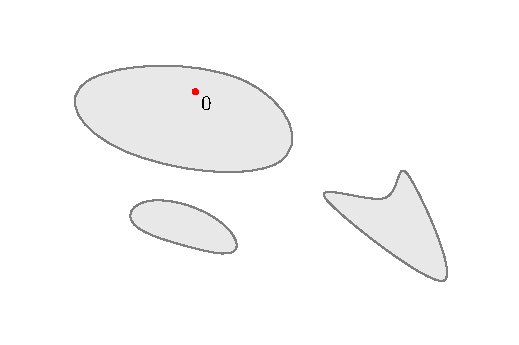
\includegraphics{nepov-lokpov.pdf}
% \caption[caption za v kazalo]{Dolg caption pod sliko}
  \caption[Primer vektorske slike.]{Za vsako točko $x$ in vsako okolico $U$ točke $x$ obstaja odprta povezana množica $V$, za katero velja $x \in V \subseteq U$.}
  \label{fig:nepov-lokpov}
\end{figure}
\end{primer}

Obstajajo pa tudi prostori, ki so povezani, vendar so lokalno nepovezani. Prepričajmo se, da temu pogoju ustreza varšavski lok. Slika~\ref{fig:vl-lok-nepovezan} prikazuje na desni strani varšavski lok, na levi strani pa je povečana okolica točke $(0, 0)$. Opazimo, da je vsaka okolica točke $(0, 0)$ nepovezana, saj vsebuje nepovezane dele varšavskega loka, ki jih lahko vidimo v povečani okolici na sliki~\ref{fig:vl-lok-nepovezan}.

\begin{figure}[h]
  \centering
  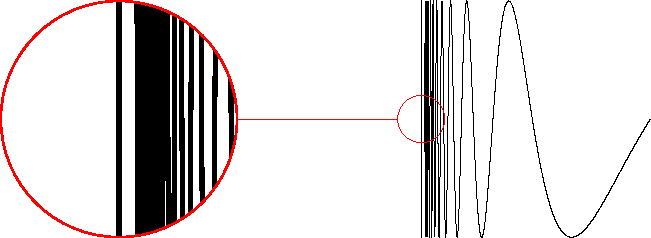
\includegraphics{varsavskilok-povecava.pdf}
% \caption[caption za v kazalo]{Dolg caption pod sliko}
  \caption[Primer vektorske slike.]{Vsaka dovolj majhna okolica točke $(0, 0)$ je nepovezana.}
  \label{fig:vl-lok-nepovezan}
\end{figure}

\begin{definicija}
Prostor $X$ je lokalno s potmi povezan prostor, če za vsako točko $ x\in X$ in vsako odprto množico $U$, ki vsebuje $x$, obstaja odprta in s potmi povezana množica $V$, ki vsebuje $x$ in je vsebovana v množici $U$.
\end{definicija}

Primer prostora, ki je lokalno s potmi povezan, je množica realnih števil ali interval v množici realnih števil. Primer prostora, ki ni lokalno s potmi povezan, pa je varšavski lok. Slika~\ref{fig:vl-lok-nepovezan} pokaže, da je vsaka dovolj majhna okolica točke $(0, 0)$ nepovezana, saj vsebuje nepovezane nepovezane dele varšavskega loka.

Varšavski lok je primer prostora, ki ni s potmi povezan in ni lokalno povezan, a je kljub temu prostor Šarkovskega.


\begin{trditev}
Varšavski lok je prostor Šarkovskega.
\end{trditev}
\begin{proof}
Varšavski lok zapišimo kot $X = C \cup A$, kjer je $A= \{0\} \times [-1, 1]$ in C krivulja $\left\{\left(x, \sin\left(\frac{\pi}{x}\right)\right), x\in [0, 1]\right\}$. Naj $f : X \to X$ zvezna preslikava, ki slika varšavski lok nazaj vase. Naj bo $x \in X$ točka s periodo $n$ za preslikavo $f$ in $m$ tako naravno število, da velja relacija $m \triangleleft n$. Pokazali bomo, da obstaja točka $y$ s periodo $m$. Ker je preslikava $f$ zvezna, se ne more zgoditi, da je $f(A) \subseteq C$ in $f(C) \subseteq A$. V tem primeru bi bila množica $f(A)$ kompaktna množica, ki nima skupne točke z množico $A$. Množici $f(A)$ in $A$ sta disjunktni zaprti podmnožici prostora $\R^2$. Ker ima prostor $\R^2$ lastnost $T_4$, obstajata disjunktni odprti množici, $U$ in $V$, za kateri velja $f(A) \subseteq U$, $f(C) \subseteq A \subseteq V$, kar predstavlja separacijo prostora $f(X)$, kar pa ni mogoče, saj je prostor $X$ povezan. Množica $f(X)$ je slika povezanega prostora z zvezno preslikavo in je tudi povezana. Če je $f(A) \subseteq C$, potem je zaradi zveznosti preslikave $f$ tudi $f(C) \subseteq C$. Ker je $X$ kompaktna množica in je slika kompaktne množice z zvezno preslikavo kompaktna, je množica $f(X)$ kompaktna povezana podmnožica množice $C$. Množica $C$ je homeomorfna intervalu, zato je tudi $f(X)$ homeromorfna intervalu, kar pomeni, da je tudi $f(X)$ prostor Šarkovskega. Zato obstaja točka $y$ s periodo $m$. Če je $f (C) \subseteq A $, potem je tudi $f (A) \subseteq A $ in vsaka periodična točka preslikave $f$ leži v $A$.  Zopet je množica $f(X)$ povezana kompaktna podmnožica homeomorfna intervalu. Torej obstaja točka $y$ s periodo $m$. 
Dokazati moramo še primer, ko je $f (A) \subseteq A $ in $f (C) \subseteq C $. Ker sta prostora $A$ in $C$ homeomorfna intervalu, sta prostora Šarkovskega, kar pomeni, da zagotovo obstaja točka $y \in X$, ki leži v isti komponenti za povezanost s potmi kot točka $x$ s periodo $m$.
\end{proof}

Pokazali smo že, da varšavski lok ni s potmi povezan prostor. V dokazu smo se prepričali, da ne obstaja pot, ki poveže ptostora $A$ in $C$. Če dodamo pot, ki poveže ta dva prostora, dobimo nov prostor, ki je s potmi povezan.


\begin{definicija}\label{def:vk}
Varšavska krožnica je topološki prostor, ki ga lahko definiramo na naslednji način:
$$S_W = \left\{\left(x, \sin\left(\frac{\pi}{x}\right)\right); 0 < x \leq 1\right\} \cup \{(0, y); -1 \leq x \leq 1\} \cup C,$$
kjer je C zvezna krivulja, ki povezuje točki $(0,-1)$ in $(1,0)$ in ne seka preostalega dela varšavske krožnice.
Množico lahko parametriziramo na naslednji način:
\[ p(t) = \begin{cases}
  (t, \sin(\frac{\pi}{t}), & \mbox{ če $t \in (0, 1) $}\\
 (\cos(\frac{3\pi x}{2}-\frac{\pi}{2})+1, \sin(\frac{3\pi x}{2}-\frac{\pi}{2})-1). & \mbox{ če $t \in [1, 2]$}\\
  (0, 2t-5), & \mbox{ če $t \in (2, 3]$.}
  \end{cases}
  \]
\end{definicija}

\begin{figure}[h]
  \centering
  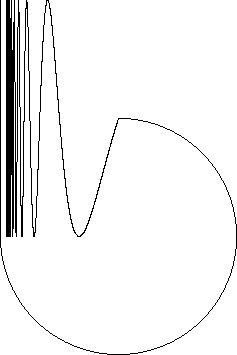
\includegraphics{varsavska_kroznica.pdf}
  \caption[Varšavska krožnica]{Slika prikazuje primer varšavske krožnice določene s predpisom $p$ iz definicije.}
  \label{fig:varsavska-kroznica}
\end{figure}

Varšavska krožnica je povezan in s potmi povezan prostor, vendar ni lokalno povezan prostor. Prepričajmo se, da je varšavska krožnica prostor Šarkovskega.

\begin{trditev} \label{trd:vk je prostor š}
Varšavska krožnica je prostor Šarkovskega.
\end{trditev}

%\begin{tikzcd}
%A \arrow{d} \arrow{r}[near start]{\phi}[near end]{\psi}
%& B \arrow[red]{d}{\xi} \\
%C \arrow[red]{r}[blue]{\eta}
%& D
%\end{tikzcd}

\begin{proof}
Interval $(0, 3]$ označimo s črko $I$, varšavsko krožnico pa z $X$. Varšavsko krožnico lahko parametriziramo z zvezno bijektivno preslikavo $p:I \to X$. Naj bo $f: X \to X$ zvezna preslikava. Ker je preslikava $p$ bijektivna, je preslikava $\widehat{f} = p^{-1} \circ f \circ p : I \to I$ dobro definirana. Trdimo, da je preslikava $\widehat{f}$ zvezna. Ker je preslikava $p$ bijekcija, imata preslikavi $f$ in $\widehat{f}$ enake periode. Ker je interval $I$ prostor Šarkovskega, je tudi $X$ prostor Šarkovskega. 

Prepričati se moramo samo še, da je preslikava $\widehat{f}$ res zvezna. Naj bo $t \in I$ poljubna točka intervala $I$ in naj bo $U \in I$ odprta okolica točke $\widehat{f}(t) = (p^{-1} \circ f \circ p)(t)$. Množico robnih točk okolice $U$ označimo z $A$. Velja $|A| \leq 2$. Ker ima $X$ lastnost $T_2$, so točke zaprte množice in zato je množica $X - p(A)$ odprta podmnožica prostora $X$, ki vsebuje točko $(f \circ p)(t)$. Povezano komponento množice $(f \circ p)^{-1}(X-p(A))$, ki vsebuje točko $t$ označimo z $W$. Množica $(f \circ p)^{-1}(X-p(A))$ je odprta podmnožica intervala $I$, saj je praslika odprte množice z zvezno preslikavo $(f \circ p)$. Ker je interval $I$ lokalno s potmi povezan, so komponente za povezanost s potmi odprte množice. Množica $W$ je zato odprta. Sedaj obravnavajmo množico $\left(p \circ \widehat{f}\right) (W) = (f \circ p)(W) \subseteq X - p(A)$. Ker je množica $W$ povezana s potmi, je množica $\left(p \circ \widehat{f} \right) (W)$ vsebovana v tisti komponenti za povezanost s potmi množice $X-p(A)$, ki vsebuje $(f \circ p)(t)$. Označimo to komponento za povezanost s potmi s črko $Z$. 

Pokažimo, da je komponenta $Z$ kar enaka $p(U)$. To je res, saj je množica $p(U)$ povezana s potmi in je zato cela vsebovana v množici $Z$. Trdimo, da komponenta za povezanost s potmi ne more vsebovati nobene druge točke. Naj bo $x$ točka iz množice $X - p(A)$, ki ne leži v množici $p(U)$. Potem točka $p^{-1}(x)$ ne leži v intervalu $U$. Definiramo pot $\gamma : [0, 1] \to X$ med točkama $p^{-1}(x)$ in $(p^{-1} \circ f  \circ p)(t)$ s predpisom 
$$\gamma(z) = (\widehat{f}(t) - p^{-1}(x)) \cdot z + p^{-1}(x).$$ 
Ker v prostoru $I$ med poljubnima točkama obstaja samo ena pot, je pot $\gamma$ edina pot v množici $I$ med točkama $p^{-1}(x)$ in $(p^{-1} \circ f \circ p)(t)$. 
Opazimo, da pot $\gamma$ v neki točki seka množico $A$. Sedaj lahko s pomočjo preslikave $p$ prenesemo pot $\gamma$ na množico $X$. Dobimo pot $\beta(z) =p((\widehat{f}(t) - p^{-1}(x)) \cdot z + p^{-1}(x))$. Tudi v množici $X$ obstaja samo ena pot od točke $x$ do točke $(f \circ p)(t)$, zato je pot $\beta$ edina pot med tema dvema točkama. Ker pot $\gamma$ seka množico $A$, pot $\beta$ seka množico $p(A)$ in ne leži cela v množici $X - p(A)$. Sklepamo, da ne obstaja pot v množici $X - p(A)$ od točke $x$ do točke $(f \circ p)(t)$, zato točki $x$ in $(f \circ p)(t)$ ne ležita v isti komponenti za povezanost s potmi. Velja $(p \circ f)(W) \subseteq p(U)$, kar implicira vsebovanost $\widehat{f}(W) = (p^{-1} \circ f \circ p)(W) \subseteq (p^{-1} \circ p)(U) = U$. Za poljubno točko $t$ in poljubno odprto okolico $U$ točke $\widehat{f}(t)$ smo našli odprto okolico $W$ točke $t$, za katero velja $\widehat{f}(W) \subseteq U$, kar dokaže zveznost preslikave $\widehat{f}$. 
\end{proof}

\begin{figure}[h]
  \centering
  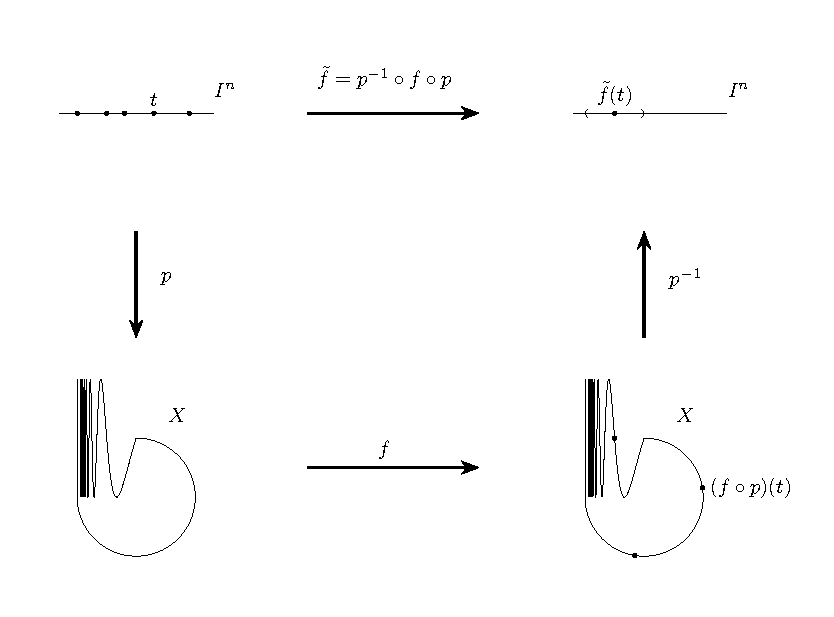
\includegraphics[scale=1.2]{vk-shark.pdf}
  \caption[Varšavska krožnica]{Skica dokaza trditve~\ref{trd:vk je prostor š}.}
  \label{fig:varšavski}
\end{figure}

\end{document}